\section[Temporally Ordering Concentration Profiles]{Temporally Ordering Concentration Profiles}

\begin{frame}{Ordering Data Temporally Using Diffusion Maps}

\begin{itemize}
\item Diffusion maps \footnote{ \tiny Coifman {\em et al}, PNAS, 2005.} (DMAPS) is a {\em nonlinear} dimensionality reduction technique.
\item DMAPS will find a parameterization of data sampled from a low--dimensional curve or manifold {\em embedded} in high--dimensional space.
\end{itemize}

	\begin{minipage}{0.45\textwidth}
	\centering
		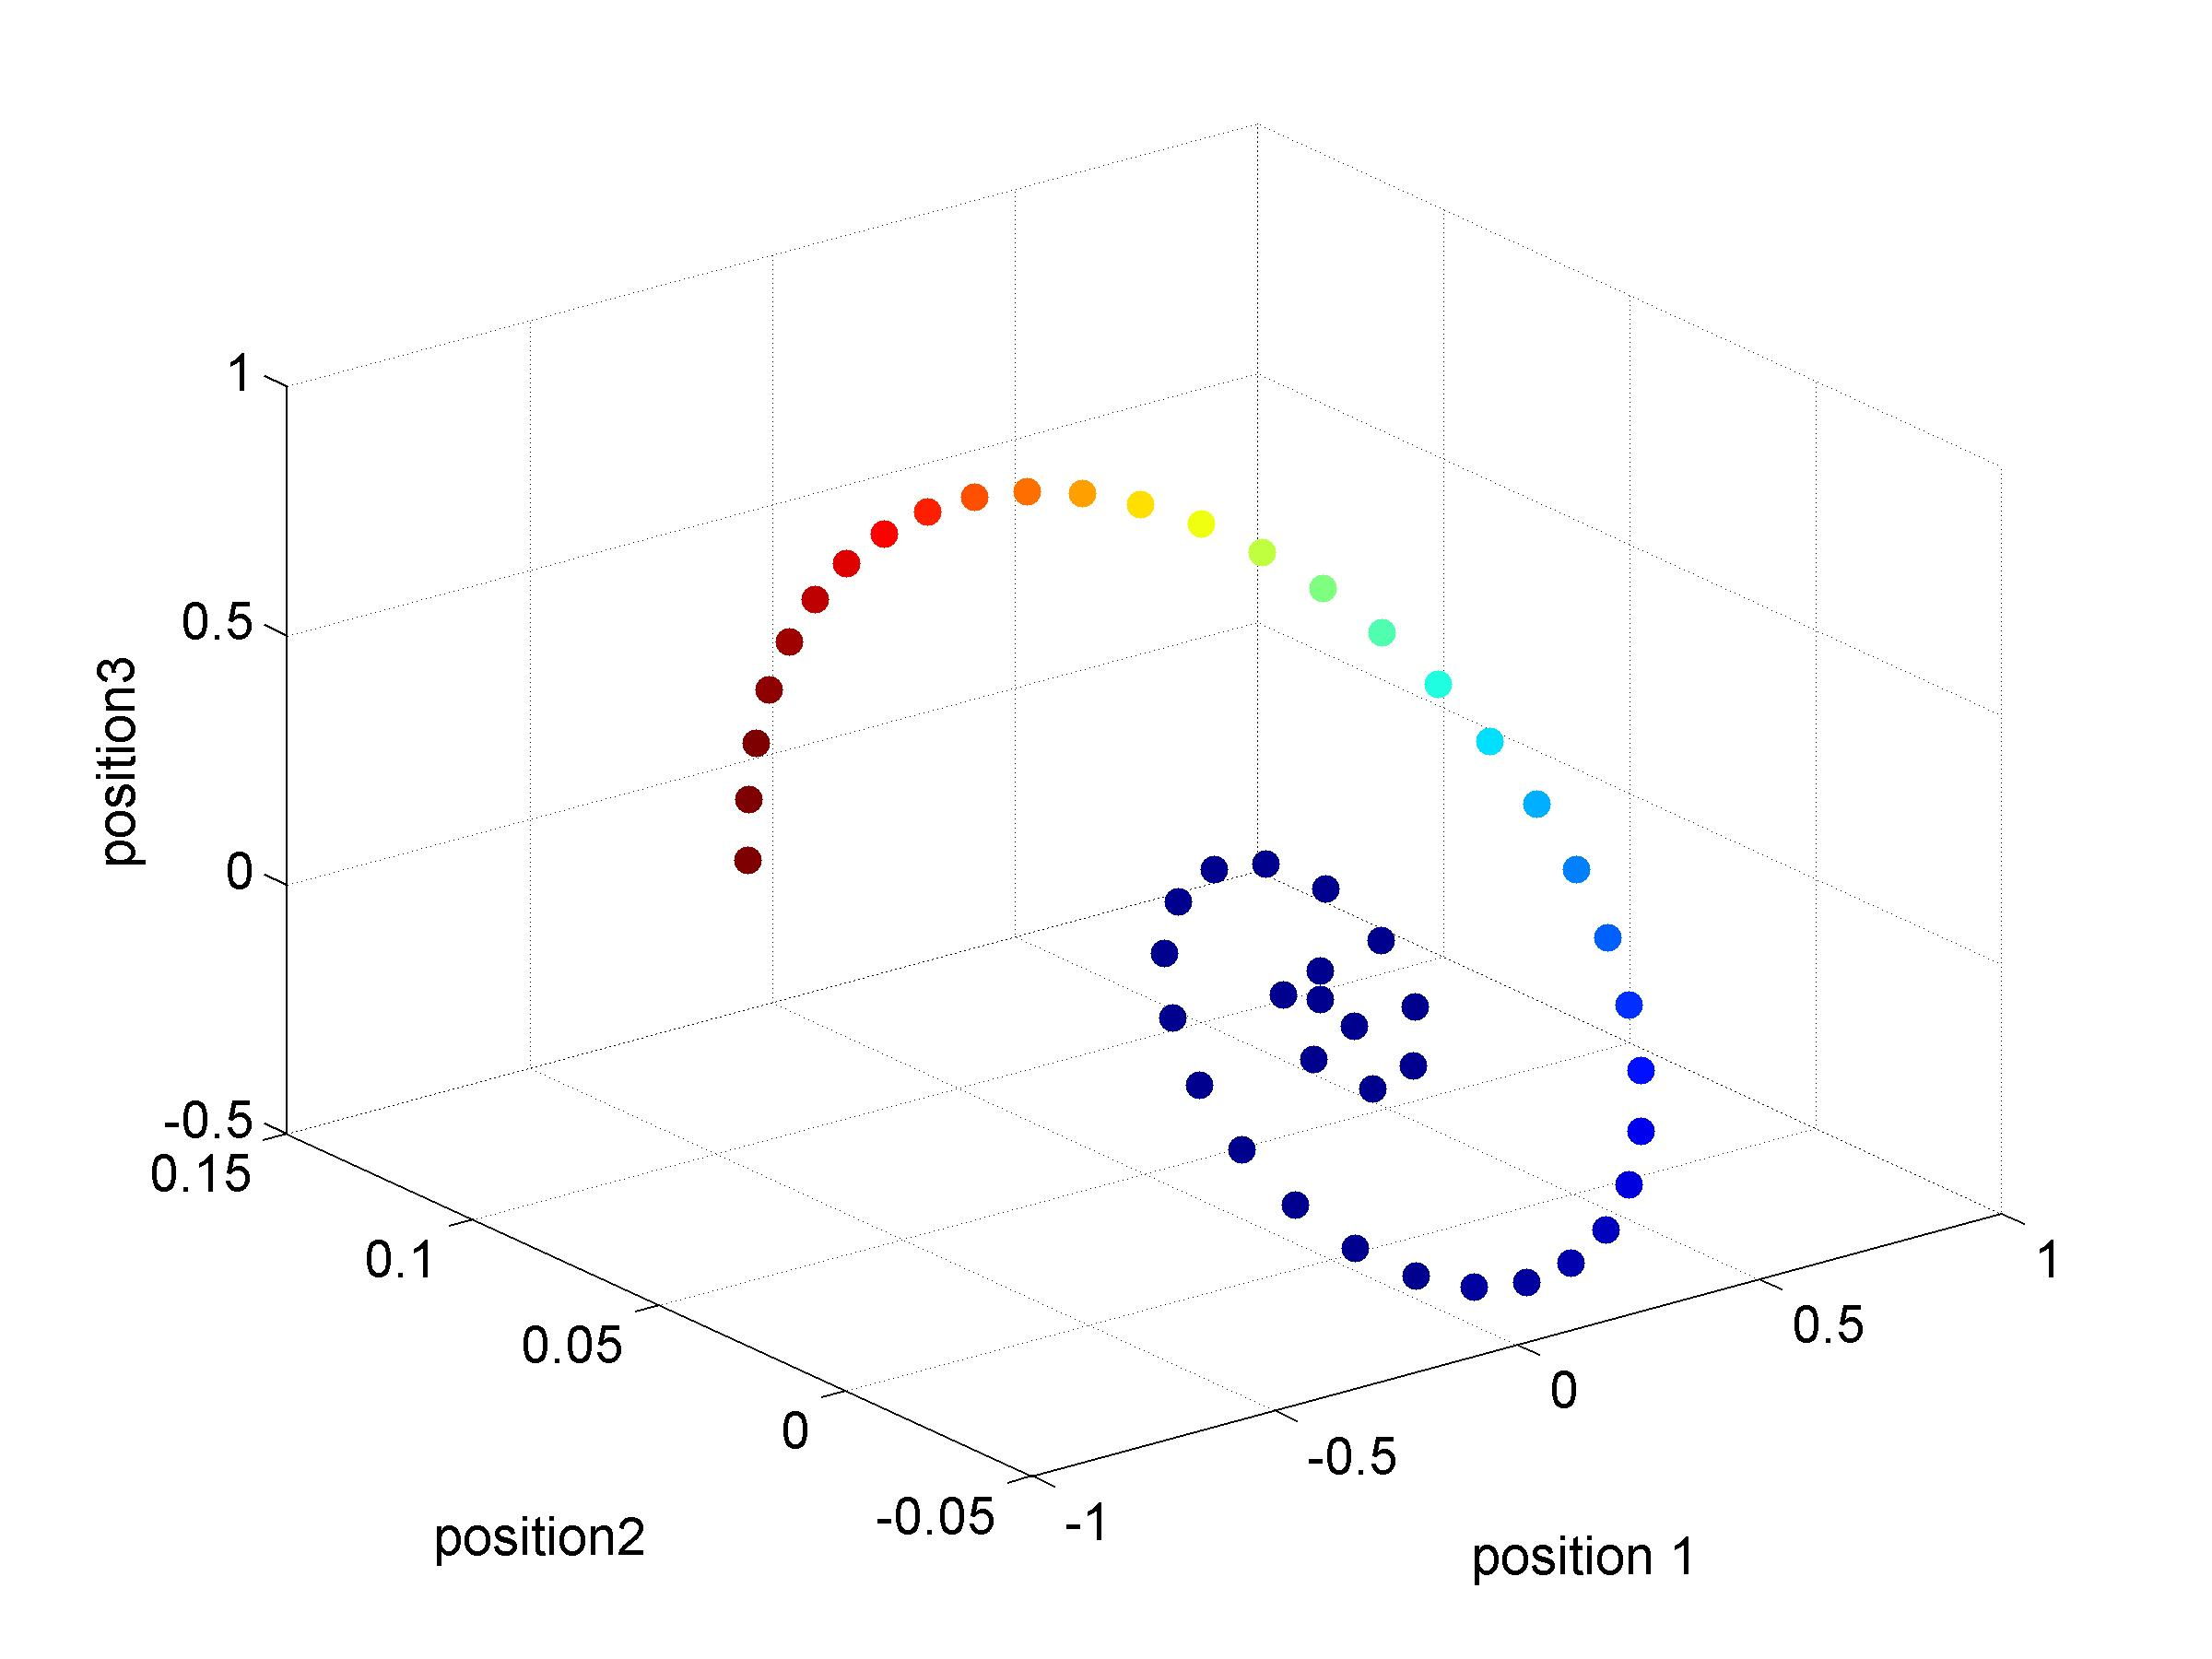
\includegraphics[width=0.7\textwidth]{dmaps_spiral.jpg}\\
		\centering
		{\scriptsize A spiral data set. The data is three--dimensional, but lies on a one--dimensional nonlinear curve. \\
		The spiral has been colored by~the~first~(non-trivial) DMAPS component. \par}
	\end{minipage}
	\hfill
	\begin{minipage}{0.5\textwidth}
		\begin{block}{DMAPS Algorithm}
		{\scriptsize 
		Calculate weight matrix $W$, where
		$$W_{ij} = exp\left( -\frac{d^2(x_i, x_j)}{\epsilon} \right).$$
		Calculate diagonal matrix $D$ with $D_{ii} = \sum_j W_{ij}.$
		
		The embedding coordinates are given by the {\bf top~eigenvectors} of $A=D^{-1}W$.
		\par}
	\end{block}
	\end{minipage}
%On the left you see data that has been ordered and colored using PCA.
%On the right you see data that has been ordered and colored using DMAPS.

%Principal component analysis \footcite{shlens2005tutorial} would not be able to order the data on the right ``correctly'', \\since the curve is one-dimensional, but non-linear.

{\small
\begin{itemize}
\item We will assume that our {\em Drosophila} data are effectively one-dimensional, and that this dimension is correlated with time. 
%
\item Therefore, ordering our data along the first direction uncovered by DMAPS will allow us to order our data in time. 
\end{itemize}
\par}

\end{frame}

\begin{frame}{Using DMAPS to Order Concentration Profiles}

	We computed the DMAPS embedding of the concentration profiles, using the Euclidean distance between concentration profiles as the distance metric. 
	
	\centering
  \begin{tikzpicture}
  	\node (unordered) {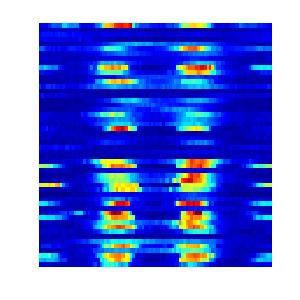
\includegraphics[width=0.4\textwidth]{data_unordered}};
  	\node[right of=unordered, node distance=0.6\textwidth] (ordered) {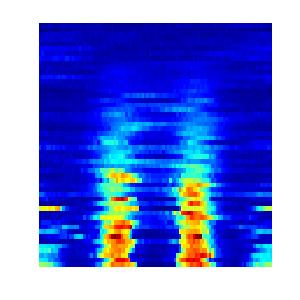
\includegraphics[width=0.4\textwidth]{data_ordered_DMAPS}};
    \draw [->] (unordered.east) -- (ordered.west) node[above,midway, text width=0.2\textwidth, align=center] {{\small Ordered using the first DMAPS coordinate \par}};    
  
  \only<2>{\node[right of=unordered, node distance=0.3\textwidth]{{\animategraphics[width=0.4\textwidth]{4}{dpERK_vdm_all_}{2}{52}}};}

  \end{tikzpicture}
  
  
\end{frame}

%\begin{frame}{Validating Our Orderings Using Membrane Thickness}
%
%\begin{itemize}
%\item We need to validate that our assumption about our data being effectively one--dimensional and monotonic in time.
%%
%\item During nuclear cycle 14, the membrane thickness is monotonic in time \footcite{lim2013kinetics, lecuit2002slam}. 
%\end{itemize}
%
%    %\vspace{0.1in}
%    \begin{tikzpicture}
%        \node (dpERK_5min) {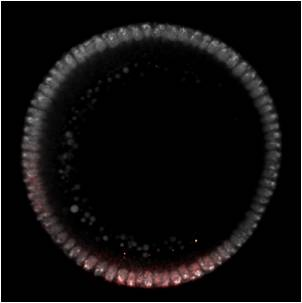
\includegraphics[width=0.1\textwidth]{dpERK_5min}};
%        \node[right=0in of dpERK_5min] (mem_5min) {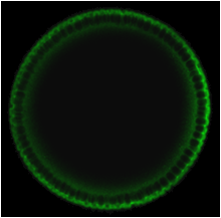
\includegraphics[width=0.1\textwidth]{membrane_5min}};
%        \node[below=0.1in of dpERK_5min] (dpERK_20min) {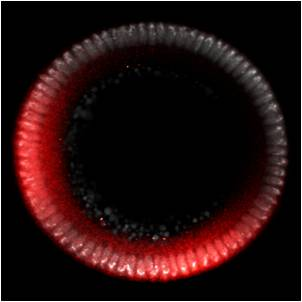
\includegraphics[width=0.1\textwidth]{dpERK_20min}};
%        \node[right=0in of dpERK_20min] (mem_20min) {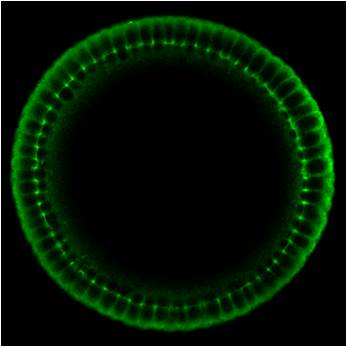
\includegraphics[width=0.1\textwidth]{membrane_20min}};
%        \node[below=0.1in of dpERK_20min] (dpERK_45min) {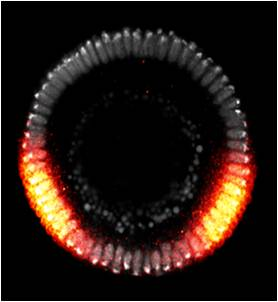
\includegraphics[width=0.1\textwidth]{dpERK_45min}};
%        \node[right=0in of dpERK_45min] (mem_45min) {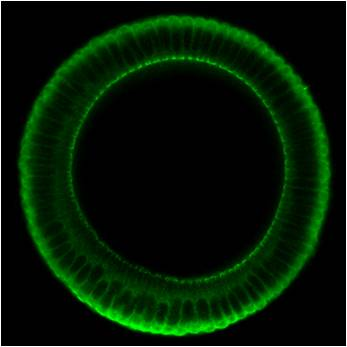
\includegraphics[width=0.1\textwidth]{membrane_45min}};
%        \node[below=0.25in of $(dpERK_45min)!0.5!(mem_45min)$, text width=0.3\textwidth, align=center](text1) {{\scriptsize \em We stain each embryo for dpERK and membrane proteins \par}};
%        \node[right=0.5in of mem_20min] (calibration) {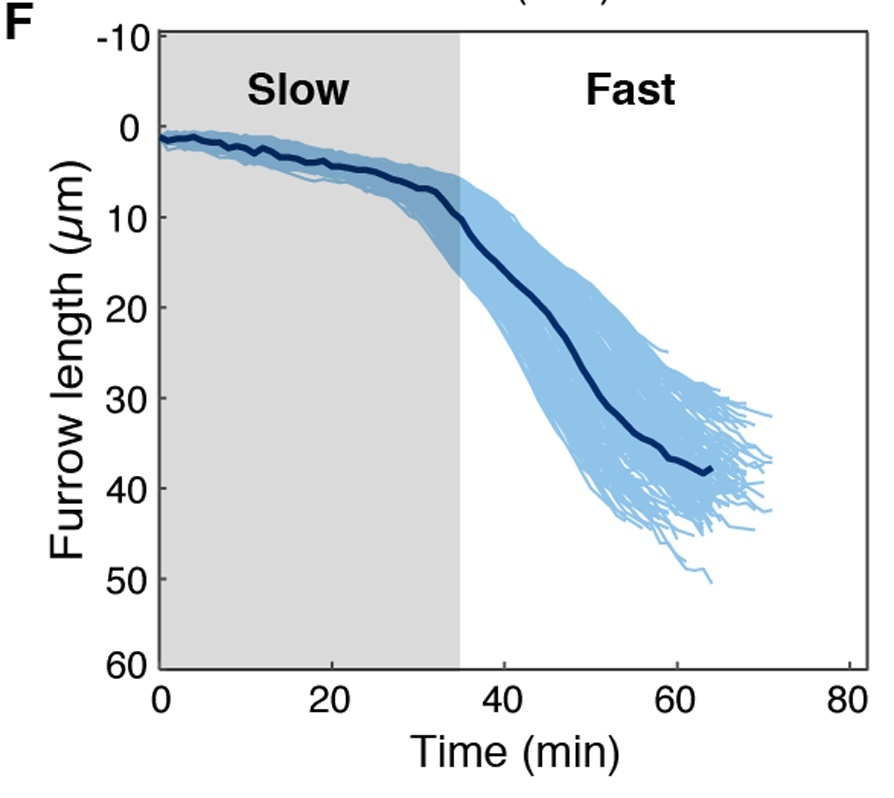
\includegraphics[width=0.3\textwidth]{calibration_curve}} edge[<-] (mem_5min) edge[<-] (mem_20min) edge[<-] (mem_45min);
%        \node[below=0in of calibration, text width=0.3\textwidth, align=center](text2) {{\scriptsize \em The membrane thickness or ``furrow length'' is monotonic in time or age of the embryo \par}};
%        \node[right=2.5in of mem_20min] (time_20) {20 minutes} edge[<-] (calibration);
%        \node[right=2.5in of mem_5min] (time_5) {5 minutes} edge[<-] (calibration);
%        \node[right=2.5in of mem_45min] (time_45) {45 minutes} edge[<-] (calibration);
%        \node[below=0in of time_45, text width=0.25\textwidth, align=center](text2) {{\scriptsize \em We can calculate the age of each embryo from the membrane thickness \par}};
%    \end{tikzpicture}
%
%We can therefore assess the quality of our orderings by plotting the rank of each data point from our DMAPS orderings against the rank obtained from ordering by membrane length. 
%
%\end{frame}


\begin{frame}{Validating DMAPS Ordering with Membrane Markers}

\begin{itemize}
\item During nuclear cycle 14, there is an {\em independent way} to measure the age of an embryo (using membrane markers).
%
\item We can therefore compare our orderings obtained from DMAPS to the orderings obtained from the membrane markers. 
\end{itemize}

	\centering
	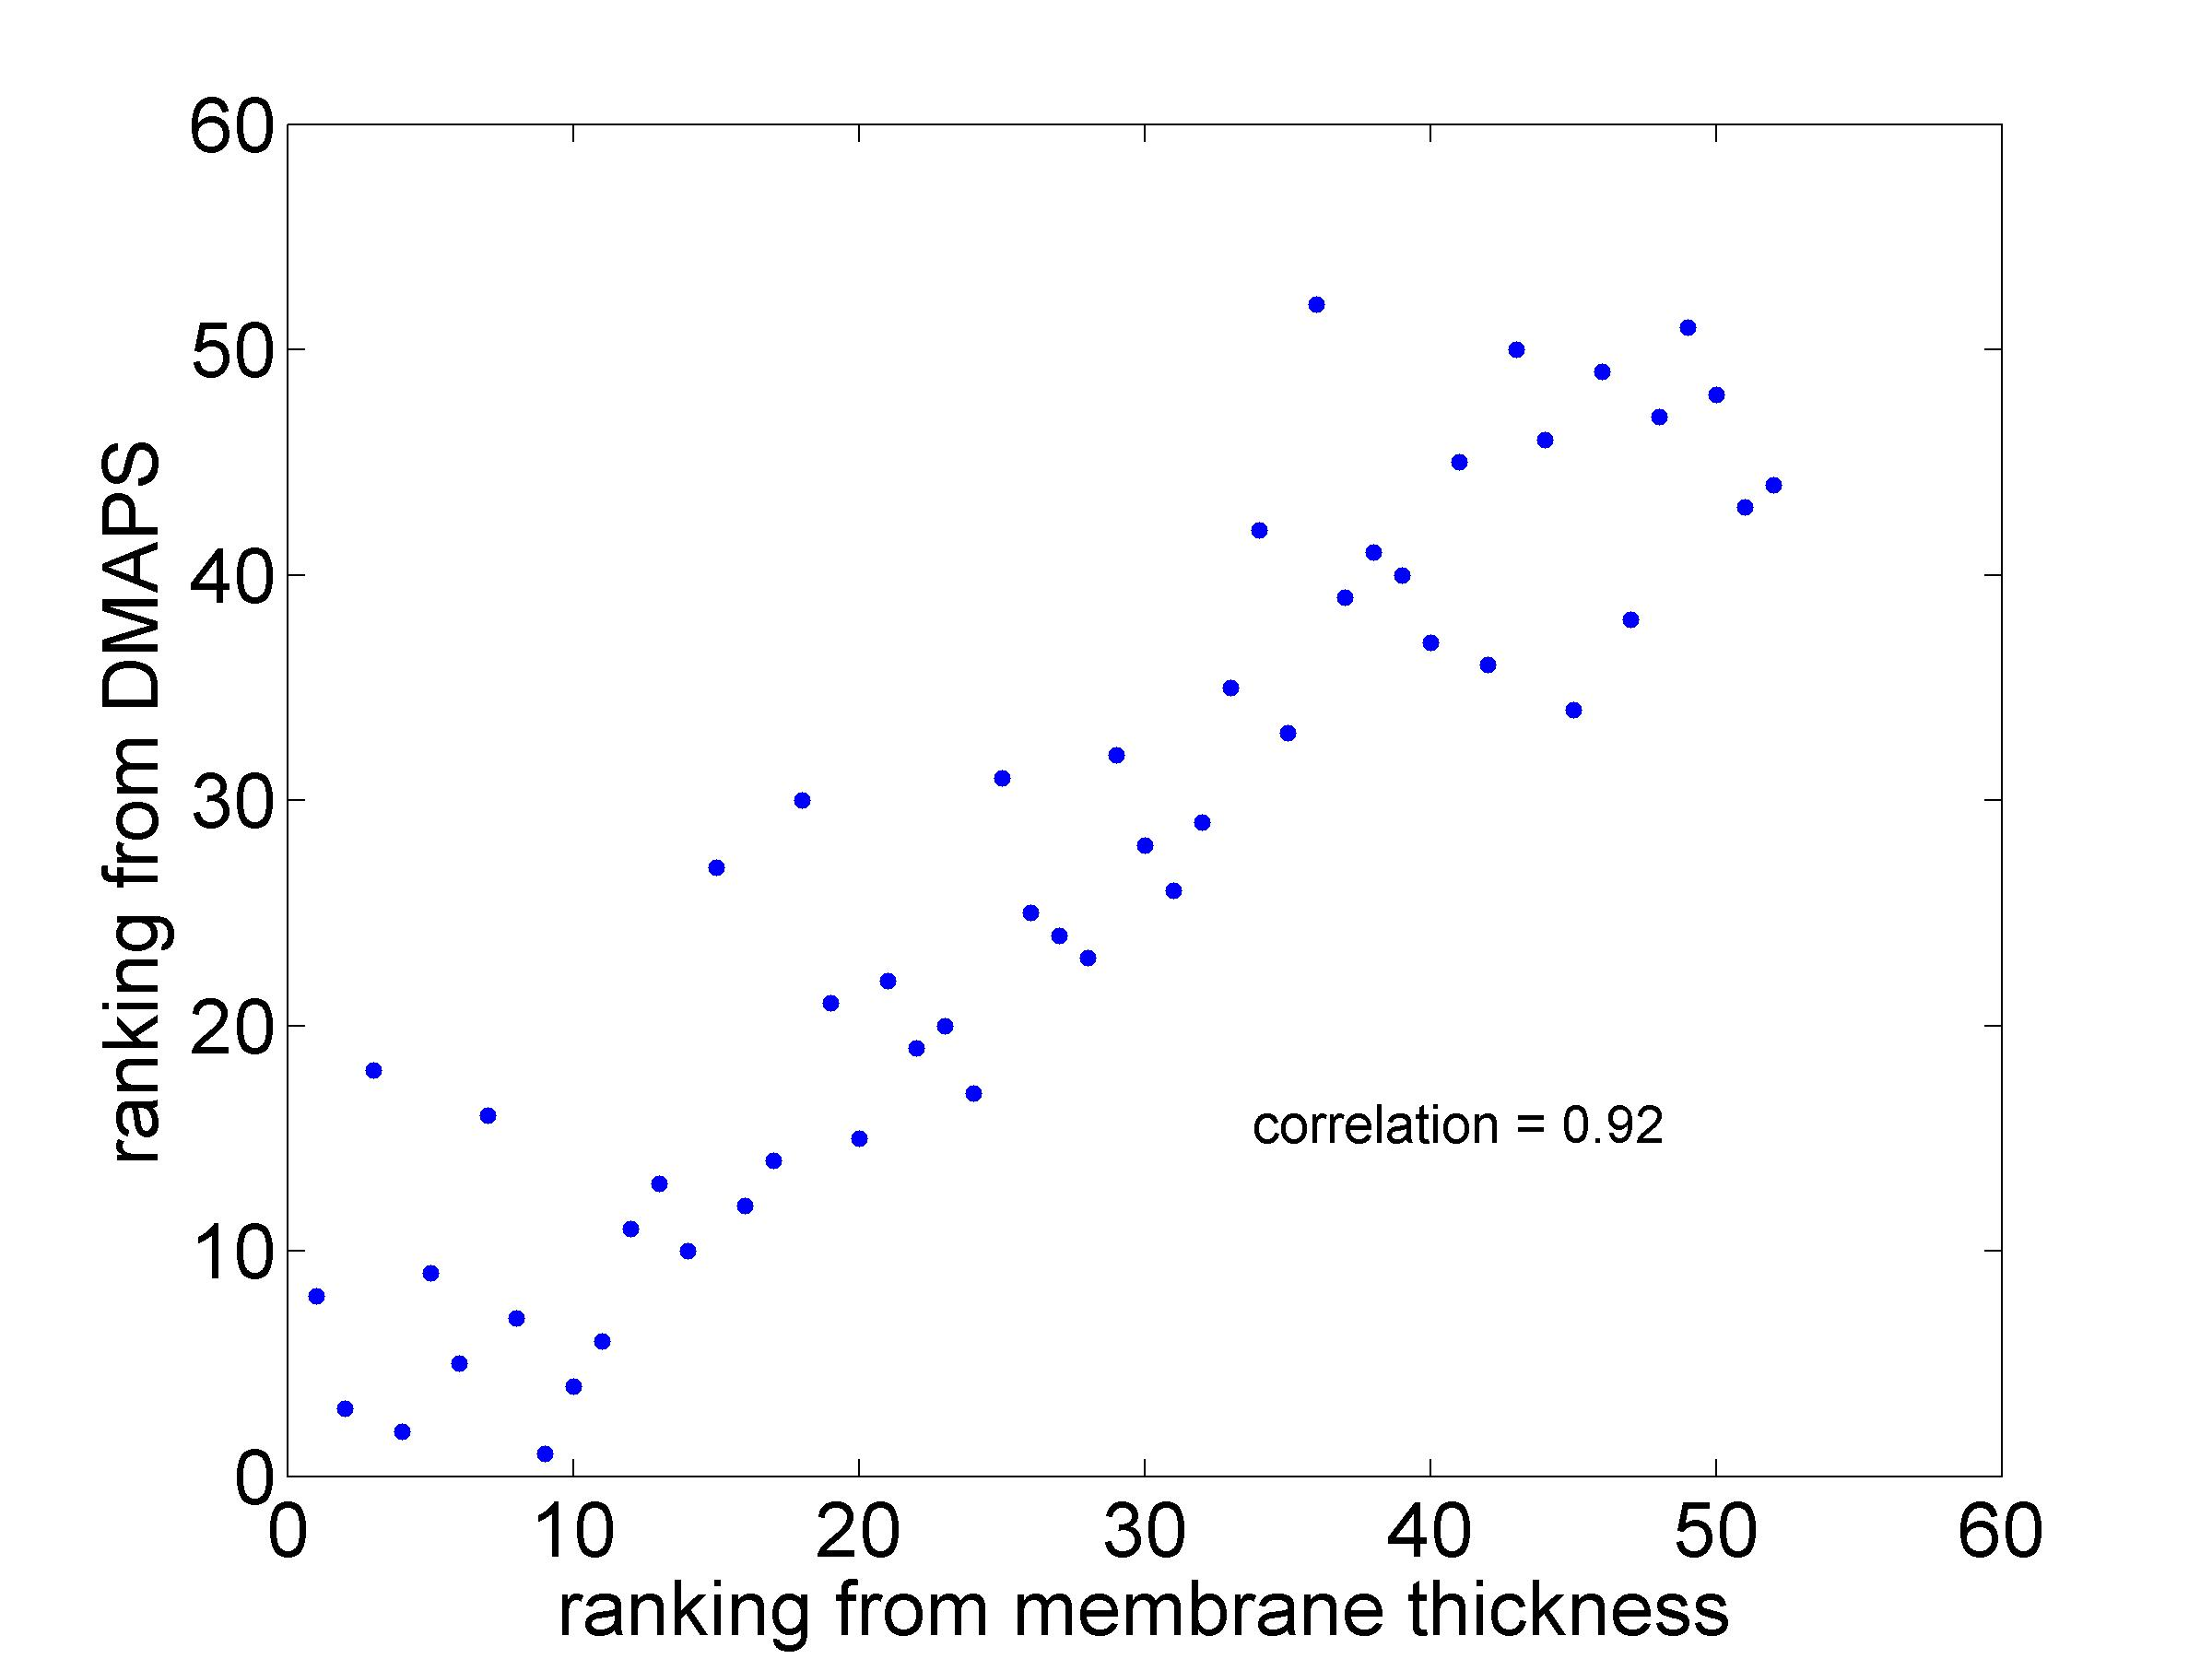
\includegraphics[width=0.5\textwidth]{DMAPS_rank_corr}	
	
The ordering obtained from DMAPS is well--correlated \\ with the ordering obtained from the membrane markers.
	
\end{frame}
